% !Mode:: "TeX:UTF-8"

\chapter{预备知识}
\label{ch:pre}



\section{图像的视觉信息抽取}



\subsection{神经网络}

\subsubsection{一般神经网络}
神经网络(neural network)的方面的研究就出现了,早起的神经网络主要是指生物学中的``生物神经网络'',在当前计算机领域特指``神经网络学习''。神经网络最基本的结构是神经元模型,神经元模型如图\ref{fig:nn-example},在这个模型中包括输入端、神经元权重(weight)、偏差(bias)、激活函数(activation function)、阀值、输出。在这个模型中,当前神经元接收其它$n$个神经元的输入,与连接权重相乘之后加上偏差,然后激活函数的处理得到激活值输出。

理想中的激活函数是如公式\ref{eq:activate-sgn},将输入值映射为输出值"1"或者"0",其中"1"对应神经元兴奋,"0"对应于神经元抑制,但是因为该阶跃函数具有不连续、不光滑等性质。因此常采用Sigmoid函数作为激活函数,一般来说激活函数是非线性的、可微的。如果不使用线性激活函数,采用线性激活函数(恒等激活函数,图例中$f(x) = x$)的话,那么神经网络只是把输入线性组合再输出,和没有采用神经网络是一样的。
\begin{equation}\label{eq:activate-sgn}
    sgn(x)=\left\{
    \begin{aligned}
    1, x\geq 0 \\
    0, x<0 \\
    \end{aligned}
    \right.
\end{equation}
例如sigmoid函数可以把$(-\infty,+\infty)$输入值映射到(0,1)区间内。常见的激活函数还有tanh(hyperbolic tangent, tanh)函数、修正线性单元(rectified linear units,ReLU)函数等等。表\ref{tab:activate-func}详细的列出了3个常用激活函数的原函数、一阶导数、以及函数的值域。其中tanh函数只是sigmoid函数向下平移再拉升的结果。并且在实际应用中,tanh的效果是好于sigmoid,因为tanh的函数值域是属于(-1,1)的,使用tanh代替sigmoid,会使得神经元输出的均值趋近于0而不是0.5,这样的结果会使得下一层的学习变得更加简单。但是对于多层的神经网络,sigmoid和tanh在极大或极小时梯度会趋近于0,会造成梯度弥散问题。但是对于ReLU 来说,当小于0时,梯度是小于0的,当大于0是,梯度是常数。ReLU激活函数在实际训练中取得了良好的效果。但是对于小于0的部分,此时的梯度为0,神经元不会训练,因此研究者们提出了LeakyReLU等激活函数解决这一问题。

前面介绍了神经元模型和各类激活函数,这里需要提到是深度神经网络、前向传播和反向传播。一个包含一个隐藏层的网络如图
\begin{table}[htpb]
  \centering
  \caption{}
  \label{tab:activate-func}
  \begin{tabular}{c|c}
    \toprule[1.5pt]
    函数名称 & 原函数 ~~~~~一阶导数$f^{'}(x)$~~~~~原函数值域 \\
    \midrule
    sigmoid函数 & $\sigma(x) = \frac{1}{1+e^{-x}}$ ~~~~ $f^{x}(x)=\sigma(x)(1-\sigma(x))$ ~~~~ (0,1) \\
    tanh函数 & $tanh(x) = \frac{e^x-e^{-x}}{e^x+e^{-x}}$ ~~~~ $f^{'}(x)=1-tanh(x)^{2}$ ~~~~ (-1,1) \\
    ReLU函数 & $relu(x) = max(0,x)$ ~~~~ $sgn(x)=\left\{\begin{aligned}1, x\geq 0 \\0, x<0 \\\end{aligned}\right.$ ~~~~ [0,+\infty)
    \bottomrule[1.5pt]
  \end{tabular}
\end{table}


\begin{figure}[htpb]
	\centering
	%	\includegraphics[width=0.48 \textwidth, trim=10 10 10 80,clip]{./pic/example_new.pdf}
	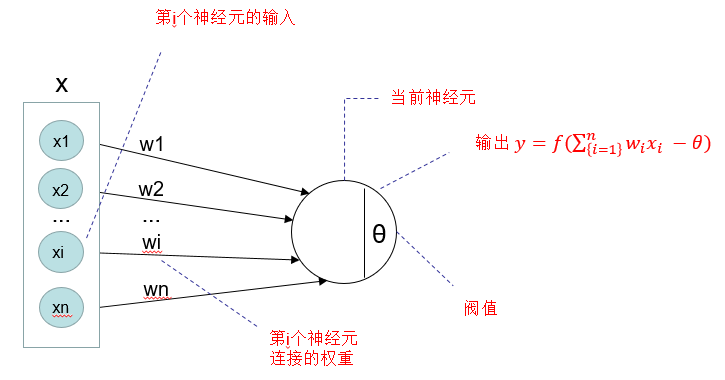
\includegraphics[width=0.95 \textwidth,clip]{nn.png}
	%\hspace{0.02\textwidth}
	%\vspace*{-0.08cm}
    \caption{神经元模型示意图}
	\vspace*{-3.5mm}
	\label{fig:nn-example}
\end{figure}
\subsubsection{卷积神经网络的介绍}
卷积神经网络(Convolutional Neural Network,CNN)是深度学习的代表算法之一,由LeCun首次实现并且应用。卷积神经网络的主要作用是提取特征,该网络受到生物学的影响,相比较与全连接神经网络,卷积神经网络的主要特性包括局部感知和参数共享。局部感知指对于具有空间特征的输入来说,每个神经元没必要知道全局的信息,只需要感知局部的信息,然后在更高层将局部的信息合并起来得到更高层的信息。对于权值共享来说,每个卷积核与位置无关,因为假设对于图像来说,其中某一部分的统计特性和其它的部分是一样的,所以对于其中的一个卷积核来说,可以应用到图像上的任何地方去。所以,局部感知和参数共享不仅能提取到更多的特征,并且能大幅度减少参数的数量。因此,卷积神经网络广泛的应用在图像、视频、音频和文本等各种模态的数据上,并且都取得了巨大的成功。

卷积神经网络的特征提取层主要包括两个模块,分别是卷积层(convolutional layer)和池化层(pooling layer),两者的顺序,一般是先通过卷积层,然后是池化层。对于卷积层,主要的作用是提取特征,卷积层的核心是卷积核(kernel),其本质还是神经元。但是卷积核的感受野和全连接的神经元是不同的,这里的感受野是局部的,并且感受野的大小由卷积核的大小控制。如图\ref{fig:con-example}所示,当前卷积核的大小是$4 \times 4$的,对于输入的图片$6 \times 6 \times 3$,其中图片输入的3为图片的通道数、$6 \times 6$为高宽,假设滑动的步骤为$1$,卷积核通过在输入图片上按照步长进行滑动并且进行对应位置的点乘运算,最后形成一个$4 \times 4$ 的特征图。以上综合起来就是卷积操作,其中$3 \times 3$就是网络的参数。按照惯例,输入的图片可以有固定的的高宽和通道数时,卷积核可以有不同的高宽,但是必须是固定的通道数,这里一般和输入的通道数一致。有多少个卷积核,最后就能得到多少个特征图(feature map)。
\begin{figure}[htpb]
	\centering
	%	\includegraphics[width=0.48 \textwidth, trim=10 10 10 80,clip]{./pic/example_new.pdf}
	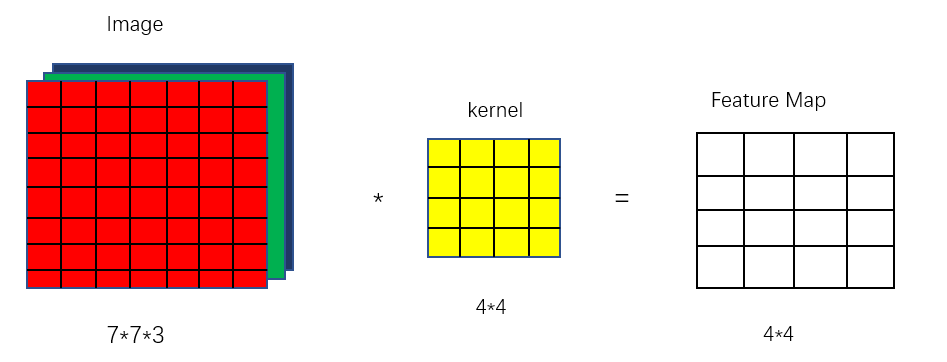
\includegraphics[width=0.95 \textwidth,clip]{conv.png}
	%\hspace{0.02\textwidth}
	%\vspace*{-0.08cm}
    \caption{卷积神经网络的卷积层示意图}
	\vspace*{-3.5mm}
	\label{fig:conv-example}
\end{figure}

对于池化层来说,主要的作用是对于卷积层输出的特征图提取主要特征,降低网络的参数,且有防止过拟合的作用。常见的池化包括平均池化(Average pooling)和和最大池化(Max pooling)。具体细节如图\ref{fig:pooling-example}所示,池化也是通过类似卷积的操作实现的,在图例中,池化也是以$2 \times 2$在特征图上进行滑动,滑动的步骤为$2$,而最大池化是选着窗口中的最大值作为输出,平均池化是选择窗口中所有值的平均值进行输出,假设输入的特征图为$C \times W \times H$ ,那么经过如图例所示的操作后得到的特征图为$C \times \frac{W}{2} \times \frac{H}{2}$。
\begin{figure}[htpb]
	\centering
	%	\includegraphics[width=0.48 \textwidth, trim=10 10 10 80,clip]{./pic/example_new.pdf}
	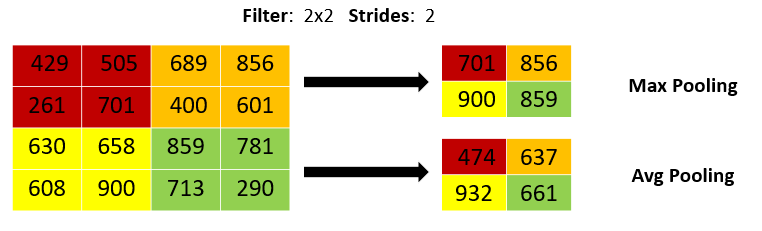
\includegraphics[width=0.95 \textwidth,clip]{pooling.png}
	%\hspace{0.02\textwidth}
	%\vspace*{-0.08cm}
    \caption{卷积神经网络的池化层示意图}
	\vspace*{-3.5mm}
	\label{fig:pooling-example}
\end{figure}

综合上述对于卷积神经网络的卷积和池化的介绍,因为每层的输入和输出都表现为特征图的形式,因此卷积神经网络可以和全连接的网络一样可以有多层,并且取得更好的效果。LeNet-5\cite{lecun1998gradient-based}是
Yang LeCun等人在$1988$年提出的,它是第一个成功应用于数字识别问题的卷积神经网络,在著名的MINIST数据集上,LeNet-5可以取得大约$99.2\%$的准确率。LeNet-5是一个经典的卷积神经网络,前5层分别是卷积层和池化层,后2层全连接层。之后于$2012$ 年提出的AlexNet\cite{DBLP:conf/nips/KrizhevskySH12},其网络结构如图\ref{fig:alexnet-example}首次使用Relu激活函数替代Sigmoid,并且验证了其在较深网络上的作用,成功解决了Sigmoid在较深网络的梯度弥散问题,虽然Relu 很早就提出了。其次,AlexNet首次在训练中使用dropout层抑制一部分激活的神经元,以避免过拟合,并且通过实践证明了效果。与此同时,模型还采用了数据增强等trick来防止过拟合,使用cuda提高训练速度。而之后提出的VGG\cite{DBLP:journals/corr/SimonyanZ14a},相比较与之前的LeNet和AlexNet,最大的特点是网络更深,具有16-19层,不包含池化和最后的softmax层。
\begin{figure}[htpb]
	\centering
	%	\includegraphics[width=0.48 \textwidth, trim=10 10 10 80,clip]{./pic/example_new.pdf}
	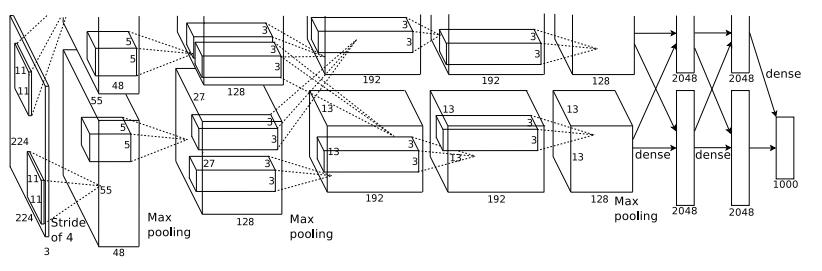
\includegraphics[width=0.95 \textwidth,clip]{alexnet.png}
	%\hspace{0.02\textwidth}
	%\vspace*{-0.08cm}
    \caption{AlexNet网络结构示意图}
	\vspace*{-3.5mm}
	\label{fig:alexnet-example}
\end{figure}
ResNet\cite{DBLP:conf/cvpr/HeZRS16}是何凯明等人(2016)提出的,针对前面网络并不能随着层数的叠加而性能的提高,ResNet首次提出了残差学习单元。如图\ref{fig:resnet-example}所示,假设模块的输入为$x$,$F(x)$指的是网络中的一系列的张量运算,假设神经网络最优的拟合结果为$H(x) = F(x) + x$,那么神经网络的最优的映射函数$F(x)$为$H(x)$和$x$之间的残差。通过不断的叠加这个模块,可以得到不断加深网络但是不降低网络性能。
\begin{figure}[htpb]
	\centering
	%	\includegraphics[width=0.48 \textwidth, trim=10 10 10 80,clip]{./pic/example_new.pdf}
	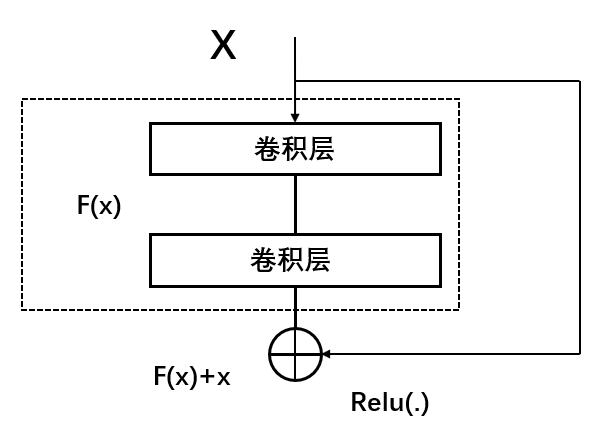
\includegraphics[width=0.95 \textwidth,clip]{resnet.png}
	%\hspace{0.02\textwidth}
	%\vspace*{-0.08cm}
    \caption{ResNet残差学习单元示意图}
	\vspace*{-3.5mm}
	\label{fig:resnet-example}
\end{figure}

综上,卷积神经网络自提出以来,得到了极大的发展,表现为新的激活函数,降低过拟合的dropout层,残差学习模块,加上cuda硬件加速的发展,我们能训练更复杂更深的神经网络,取得更好的性能。

\subsection{物体检测与识别}

在社会关系识别的任务中,有一个重要的模块是利用物体识别模型得到人的场景信息,即采用物体识别模型识别去当前图片中包含了哪些物体,得到该物体在图片的区域。物体识别的模型包括Ross等人提出的RCNN\cite{DBLP:conf/cvpr/GirshickDDM14},fast-RCNN\cite{DBLP:conf/iccv/Girshick15},以及Ren等人(2016)\cite{DBLP:conf/nips/RenHGS15}提出的faster-RCNN。前面提到的三个模型都是基于区域的物体检测模型,RCNN\cite{DBLP:conf/cvpr/GirshickDDM14}首次提出在目标图像中有多个目标框,然后判断目标框是否包含物体,具体的检测步骤如下:
(1)其中采用选择性搜索的方法得到图片中的所需要的目标框区域,将得到的区域调整为卷积神经网络输入的消息。
(2)利用一个预训练好的卷积神经网络,提取第一步得到的区域中的特征。
(3)将第二步中得到的特征当作一个线性SVM的输入,得到物体的类别,另外训练一个线性回归模型得到物体的目标框。
RCNN的主要缺点是对于一张图片中的每个感兴趣区域,需要遍历提取其中的特征,然后依次执行物体的分类和物体框的回归,需要耗费较多时间。由于全卷积和池化层不改变某个区域在特征图和原图的位置,因此fast-RCNN 在RCNN 的基础上提出了ROI(region of interest) 池化层,将图片输入到卷积神经网络中,对于特征图上的区域,经过ROI池化层进行调整,然后再继续之后的全连接层和一个线性回归层进行分类和目标框的确定。综上,fast-RCNN 较大程度上提高了物体检测的性能。由于fast-RCNN 在大数据集上的表现依然不能满足实际的需求,因为RCNN和fast-RCNN均采用选择性搜索的方法得到所需要的区域,这个步骤是比较耗费时间。因此faster-RCNN提出RPN(region proposal network),RPN主要网络包括两部分,一部分主要是对生成的anchors进行判断是foreground还是background,其中foreground代表目标,另外一部分主要是对检测框的位置进行调整。经过RPN网络后得到候选区域,再利用ROI池化得到特征向量进行物体类别的判断和物体框的进一步精确判断。

综上,以上的篇幅主要是回顾了在社会关系检测的工作中,有用的物体检测方法和一些相关工作。结论是得益于GPU等硬件设备的发展,物体识别领域的算法也得到了快速的发展,尤其是随着特征提取模块的发展,卷积网络越来越深,能学习到更多更丰富的特征。对于一幅图片,我们能在得到更多的、更准确的物体框和类别。

\section{社会关系检测}
本章将回顾社会关系检测领域的一些相关工作,并且对于消息传递机制的介绍,以及消息传递机制的相关工作的一些介绍。

\subsection{已有工作的简单介绍}

社会关系检测是社交网络的一个基础,社会关系检测作为一个重要的多学科问题,在计算机视觉领域受到越来越多的关注。随着这个问题被提出以来,有大量的工作用于从图片中抽取两个人之间的社会关系。主要有Zhang等人(2015)\cite{DBLP:conf/iccv/ZhangLLT15}提出的利用面部表情、年龄、性别、姿势等多种特征的联合模型。Li等人(2017)\cite{DBLP:conf/iccv/LiWZK17}提出的多次观察的Dual-glance模型。以及Wang等人(2018)\cite{DBLP:conf/ijcai/WangCRYCL18}提出的基于常识知识的深度推理模型GRM。

Zhang等人提出的模型认为从心理学的角度出发,认为人的关系主要由人的面部表情的一些特点决定的。首先,模型设计了一个基准模型用于提取图片中两个人对的特征,对于两个人对,基准模型采用共享参数的深度卷积网络(DCN),利用DCN提取得到的特征分别记为$x^r,x^l$,并且$\forall x^r,x^l \in R^{2048 \times 1}$,经过一个权重矩阵$\mathbf{W} \in R^{4096 \times 256}$得到特征向量$x_t$。对于已经标注好的人脸图片两个人脸分别为和,利用DCN 提取得到的特征分别记为和,并且。除了图片中本来的特征,模型利用了两张人脸在图片的空间信息。1)两张人脸的位置分别表示为${x^l,y^l,w^l,h^l,x^r,y^r,w^r,h^r}$,其中$x-,y-$是左上角的坐标,$w,h$ 分别是两个人脸包围盒的宽度和高度。2)人脸的相对位置$\frac{x^l-x^r}{w^l},\frac{y^l-y^r}{h^l}$。3)人脸之间的比例$\frac{w^l}{w^r}$。以上的三项空间特征会和DCN得到的$x_t$拼接来学习得到关系类别。
\begin{figure}[htpb]
	\centering
	%	\includegraphics[width=0.48 \textwidth, trim=10 10 10 80,clip]{./pic/example_new.pdf}
	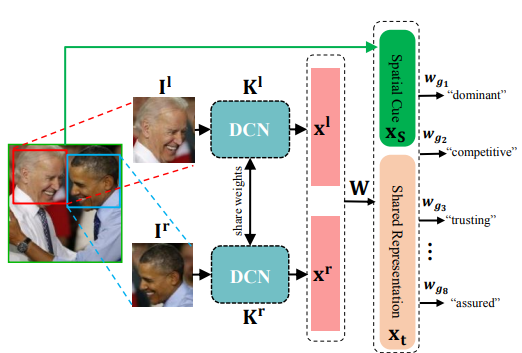
\includegraphics[width=0.75 \textwidth,clip]{1.png}
	%\hspace{0.02\textwidth}
	%\vspace*{-0.08cm}
    \caption{zhang的模型}
	\vspace*{-3.5mm}
	\label{fig:model_zhang}
\end{figure}
\looseness=-1
除此之外,$\mathbf{w_{gi}}$,$\mathbf{W}$,$\mathbf{K^l}$,and $\mathbf{K^r}$可以采用标准的正太分布初始化。结合之前符号的定义,该模型损失函数定义如下:
\begin{equation}
\begin{split}
     arg\max \limits_{\Omega} p({\mathbf{w}_{g_i}}_{i=1}^8, \mathbf{W},\mathbf{K}^r | \mathbf{g},\mathbf{x}_t,\mathbf{x}_s,\mathbf{I}^r,\mathbf{I}^l) \propto \\
     (\sum_{i=1}^{8}p(g_i|x_t,x_s)p(w_(g_i)))(\sum_{j=1}{K}p(k_j^l)p(k_j^r))p(\mathbf(W)), \\
     s.t. \mathbf{K}^r = \mathbf{K}^l
\end{split}
\end{equation}
基于以上的工作,该模型同样认为人的面部属性对最终的关系预测可以起到关键的作用。

Li等人\cite{DBLP:conf/iccv/LiWZK17}在前面的工作,针对社会检测的任务提出了包含两个关系粒度的数据集,PISC\cite{DBLP:conf/iccv/LiWZK17}。该工作首次提出了利用图片中的场景来协助预测两个人之间的关系,场景具体表示为该图片中的物体。直观来说,如果一幅图片中包含电脑桌子等物体,那么大概率是``同事''关系。模型分为两个模块,first glance和second glance,first glance的输入为一张图片$\mathbf{I}$ 和两个人身体的包围盒。针对图片$I$,首先修剪出3个小块,前两个小块分别覆盖住两个人,$p_1$和$p_2$,第三个小块覆盖两个人,表示为$p_{u}$。这三个小块的像素被修正为$224 \times 224$大小,作为后续三个CNNs 网络的输入

